\section{显示字符的toy
bootloader}\label{ux663eux793aux5b57ux7b26ux7684toy-bootloader}

\subsection{实验目标}\label{ux5b9eux9a8cux76eeux6807}

操作系统是一个软件,也需要通过某种手段加载并运行它。在这里我们将通过另外一个更加简单的软件-bootloader来完成这些工作。为此,我们需要完成一个能够切换到x86的保护模式并显示字符的bootloader,为将来启动操作系统做准备。proj1提供了一个非常小的bootloader,整个bootloader的大小小于512个字节,这样才能放到硬盘的主引导扇区中。
\textgreater{} 这里对x86的保护模式不必太在意,后续会进一步讲解

通过分析和实现这个bootloader,读者可以了解到: * 与操作系统原理相关 *
I/O设备管理:设备管理的基本概念,涉及简单的信息输出 *
内存管理:基于分段机制的存储管理,x86的实模式/保护模式以及切换到保护模式的方法
* 计算机系统和编程 * 硬件 * PC加电后启动bootloader的过程 *
通过串口/并口/CGA输出字符的方法 * 软件 * bootloader的文件组成 *
编译运行bootloader的过程 * 调试bootloader的方法 *
在汇编级了解栈的结构和处理过程

\subsection{proj1概述}\label{proj1ux6982ux8ff0}

\subsubsection{实现描述}\label{ux5b9eux73b0ux63cfux8ff0}

proj1实现了一个简单的bootloader,主要完成的功能是初始化寄存器内容,完成实模式到保护模式的转换,在保护模式下通过PIO方式控制串口、并口和CGA等进行字符串输出。

\subsubsection{项目组成}\label{ux9879ux76eeux7ec4ux6210}

{[}要点(非OSP):bootloader的编译生成过程{]}
lab1中包含的第一个工程小例子是proj1:一个可以切换到保护模式并显示字符串的bootloader。proj1的整体目录结构如下所示:

\begin{lstlisting}
    proj1 /
    |-- boot
    |   |-- asm.h
    |   |-- bootasm.S
    |   `-- bootmain.c
    |-- libs
    |   |-- types.h
    |   `-- x86.h
    |-- Makefile
    `-- tools
        |-- function.mk
        |-- gdbinit
        `-- sign.c

    3 directories, 9 files
\end{lstlisting}

其中一些比较重要的文件说明如下: * bootasm.S
:定义并实现了bootloader最先执行的函数start,此函数进行了一定的初始化,完成了从实模式到保护模式的转换,并调用bootmain.c中的bootmain函数。
*
bootmain.c:定义并实现了bootmain函数实现了通过屏幕、串口和并口显示字符串。
*
asm.h:是bootasm.S汇编文件所需要的头文件,主要是一些与X86保护模式的段访问方式相关的宏定义。
* types.h:包含一些无符号整型的缩写定义。 * x86.h:一些用GNU
C嵌入式汇编实现的C函数(由于使用了inline关键字,所以可以理解为宏)。 *
Makefile和function.mk:指导make完成整个软件项目的编译,清除等工作。 *
sign.c:一个C语言小程序,是辅助工具,用于生成一个符合规范的硬盘主引导扇区。
* gdbinit:用于gdb远程调试的初始命令脚本

从中,我们可以看出bootloader主要由bootasm.S和bootmain.c组成,当你完成编译后,你会发现这个bootloader只有区区的3百多字节。下面是编译运行bootloader的过程。

\begin{quote}
【提示】bootloader是一个超小的系统软件,在功能上与我们一般的应用软件不同,主要用于硬件简单初始化和加载运行操作系统。在编写bootloader的时候,需要了解它所处的硬件环境(比如它在内存中的起始地址,它的储存空间的位置和大小限制等)。而这些是编写应用软件不太需要了解的,因为操作系统和编译器帮助应用软件考虑了这些问题。
\end{quote}

\subsubsection{编译运行}\label{ux7f16ux8bd1ux8fd0ux884c}

\textbf{【实验 编译运行bootloader】}

在proj1下执行make,在proj1/bin目录下可生成一个ucore.img。ucore.img是一个包含了bootloader或OS的硬盘镜像,通过执行如下命令可在硬件虚拟环境
qemu中运行bootloader或OS:

\begin{lstlisting}
  make                     //生成bootloader和对应的主引导扇区
  make qemu          //通过qemu硬件模拟器来运行bootloader
  make clean          //清除生成的临时文件,bootloader和对应的主引导扇区
\end{lstlisting}

%\begin{figure}[htbp]
%\centering
%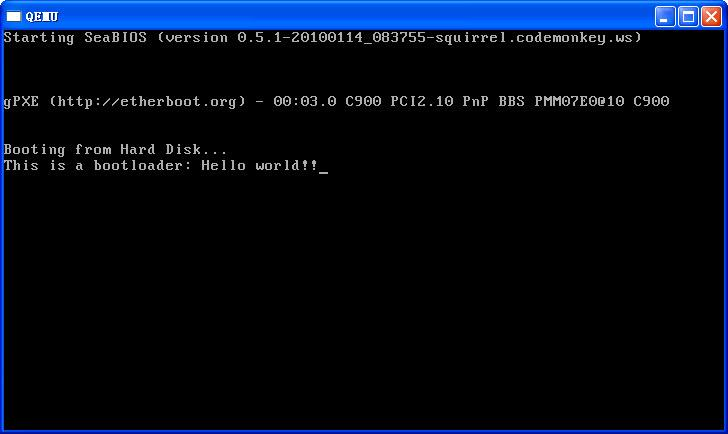
\includegraphics{figures/qemu_cha1.jpg}
%\caption{qemu\_img}
%\end{figure}

我们除了需要了解bootloader的功能外,还需要进一步了解bootloader的编译链接和最终执行码的生成过程,从而能够清楚生成的代码是否是我们所期望的。proj1中的Makefile是一个配置脚本,make软件工具能够通过Makefile完成管理bootloader的C/ASM代码生成执行码的整个过程。Makefile的内容比较复杂,不过读者在前期只需会执行make
{[}参数{]}来生成代码和清除代码即可。对于本实验的make的执行过程如下所示:

\begin{lstlisting}
    1. gcc -O2 -o tools/sign tools/sign.c
    2. i386-elf-gcc -fno-builtin -Wall -MD -ggdb -m32 -fno-stack-protector -O -nostdinc -Iinclude -Iinclude/x86 -c bootloader/bootmain.c -o obj/bootmain.o
    3. i386-elf-gcc -fno-builtin -Wall -MD -ggdb -m32 -fno-stack-protector -nostdinc -Iinclude -Iinclude/x86 -c bootloader/bootasm.S -o obj/bootasm.o
    4. i386-elf-ld  -N -e start -Ttext 0x7C00 -o obj/bootblock.o obj/bootasm.o obj/bootmain.o
    5. i386-elf-objdump -S obj/bootblock.o > obj/bootblock.asm
    6. i386-elf-objcopy -S -O binary obj/bootblock.o obj/bootblock.out
    7. sign.exe obj/bootblock.out obj/bootblock
       obj/bootblock.out size: 380 bytes
       build 512 bytes boot sector: obj/bootblock success!
    8. dd if=/dev/zero of=obj/ucore.img count=10000
       10000+0 records in
       10000+0 records out
       5120000 bytes (5.1 MB) copied, 0.509 s, 10.1 MB/s
    9. dd if=obj/bootblock of=obj/ucore.img conv=notrunc
       1+0 records in
       1+0 records out
       512 bytes (512 B) copied, 0.011 s, 46.5 kB/s
\end{lstlisting}

\textbf{这9步的含义是:}

\begin{lstlisting}
1. 编译生成sign执行程序,用于生成一个符合规范的硬盘主引导扇区;
2. 用gcc编译器编译bootmain.c,生成ELF格式的目标文件bootmain.o;
3. 用gas汇编器(gcc只是一个包装)编译bootasm.S,生成ELF格式的目标文件bootasm.o;
4. 用ld链接器把bootmain.o和bootasm.o链接在一起,形成生成ELF格式的执行文件bootblock.o;
5. 目标文件信息导出工具objdump反汇编bootblock.o,生成bootblock.asm,通过查看bootlock.asm内容,可以了解bootloader的实际执行代码;
6. 文件格式转换和拷贝工具objcopy把ELF格式的执行文件bootblock.o转换成binary格式的执行文件bootblock.out;
7. 通过sign执行程序,把bootblock.out(本身大小需要小于510字节)扩展到512字节,形成一个符合规范的硬盘主引导扇区bootblock;
8. 设备级转换与拷贝工具dd生成一个内容都为“0”的磁盘文件ucore.img;
9. 设备级转换与拷贝工具dd进一步把bootblock覆盖到ucore.img的前512个字节空间中,这样就可以把ucore.img作为一个可启动的硬盘被硬件模拟器qemu使用。
\end{lstlisting}

如果需要了解Makefile中的内容,需要进一步看看附录``ucore实验中的常用工具''一节。
